\section{Coloring}
\begin{definition}
    Let $k\in \mathbb{N}$. A (proper) \textbf{$k$-vertex-coloring} ($k$-coloring) of a graph $G$ is a function $c: V(G) \to \{1, 2, \dots, k\}$ such that for every edge $\{u,v\} \in E(G)$, we have $c(u) \neq c(v)$. The \textbf{chromatic number} $\chi(G)$ of a graph $G$ is the smallest integer $k$ such that $G$ has a proper $k$-coloring. We call $G$ \textbf{colorable} if it has a $k$-vertex-coloring. \\
    Write $\Delta(G)$ for the maximum degree of a vertex in $G$.
\end{definition}
\begin{lemma}
    Let $G$ be a graph. Then $\chi(G) \leq \Delta(G) + 1$.
\end{lemma}
\begin{proof}
    Order the vertices of $G$ as $v_1, v_2, \dots, v_n$. We will color the vertices in this order. When we come to color $v_i$, it has at most $\Delta(G)$ neighbors, so there are at most $\Delta(G)$ colors that are forbidden for $v_i$. Since we have $\Delta(G) + 1$ colors available, there is always at least one color that we can use to color $v_i$.
\end{proof}
\begin{remark}
    The bound $\chi(G) \leq \Delta(G) + 1$ is tight with equality for exactly the complete graphs $K_n$ and the odd cycles $C_{2k+1}$. 
\end{remark}
\begin{lemma}
    Let $G$ be a (connected) graph. If there is $v\in V(G)$ such that $\deg_G(v) < \chi(G)$, then $G$ has a coloring with $\Delta(G)$ colors.
\end{lemma}
\begin{proof}
    Proof by Induction on $|V(G)|$.\\
    Base case: If $|V(G)| = 1$, then $\chi(G) = 1$ and $\Delta(G) = 0$, so the statement holds.\\
    Induction step: Assume the statement holds for all graphs with fewer than $n$ vertices, and let $G$ be a graph with $n$ vertices. Let $v\in V(G)$ such that $\deg_G(v) < \chi(G)$. Consider the graph $G' = G - v$. Since $G'$ has fewer vertices than $G$, by the induction hypothesis, we have $\chi(G') \leq \Delta(G')$. Now lets look at two cases:\\
    ($1$) $\exists w\in V(G)$ such that $\deg_{G}(w) = \Delta(G)$ and $w$ is a neighbour of $v$ in $G$ and there is no $w' \in V(G')$ with $\deg_{G}(w') = \Delta(G)$ not a neighbour of $v$. Then it follows that $\Delta(G)=\Delta(G')+1=\chi(G')+1$ and $\chi(G)=\chi(G')+1$. Therefore $\Delta(G)=\chi(G)$.\\
    ($2$) There is no $w\in V(G)$ with $\deg_{G}(w) = \Delta(G)$ s.t. $w$ is a neighbour of $v$ in $G$. Then $\Delta(G)=\Delta(G')$ and $\chi(G)=\chi(G')$. Therefore $\Delta(G)=\chi(G)$.
     \begin{center}
        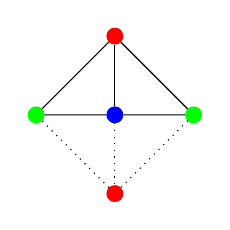
\begin{tikzpicture}[
            vertex/.style={circle, draw, fill=gray!20, minimum size=2mm, inner sep=0pt}
        ]
            \node[vertex,red] (a) at (0,2) {};
            \node[vertex,blue] (b) at (0,1) {};
            \node[vertex,red] (c) at (0,0) {};
            \node[vertex,green] (d) at (1,1) {};
            \node[vertex,green] (e) at (-1,1) {};
           
            \draw (a)--(b);
            \draw (a)--(d)--(b);
            \draw (a)--(e)--(b);
            \draw[dotted] (d)--(c)--(e);
            \draw[dotted] (b)--(c);

        \end{tikzpicture}
        \end{center}
\end{proof}
\begin{theorem}[Brooks' Theorem]
    Let $G$ be a connected graph. If $G$ is neither an odd cycle nor a complete graph, then $\chi(G) \leq \Delta(G)$.
\end{theorem}
\begin{proof}
    $\Delta(G)=0$: Then $G$ is a single vertex and therefore complete.\\
    $\Delta(G)=1$: Then $G$ is a path and therefore complete.\\
    $\Delta(G)=2$: Then $G$ is a cycle. If $G$ is an odd cycle, then $\chi(G)=3=\Delta(G)+1$. If $G$ is an even cycle, then $\chi(G)=2=\Delta(G)$.\\
    Let $\Delta(G)\geq 3$\\
    By Lemma ("$5.4$"), we may assume that $G$ is $\Delta(G)$-regular ($\forall v\in V(G)$, $\deg_G(v)=\Delta(G)$).\\
    \begin{enumerate}
        \item $\exists v\in V(G)$ such that $G-v$ is disconnected. Then $G-v$ has at least two components. Let $C_1,...C_k$ be the components of $G-v$, and let $G_i=G[V(C_i)\cup\{v\}]$. $G_i$ is connected, $\Delta(G_i)=\Delta(G)$ and since $\deg_{G_i}(v)<\deg_G(v)=\Delta(G)\implies$ (by Lemma "$5.4$") we can color $G_i$ with $\Delta(G)$ colors. Fix such a coloring and then permute the colors s.t. $v$ always has the same color. Then this is a coloring of $G$ with $\Delta(G)$ colors.\\
            \begin{center}
            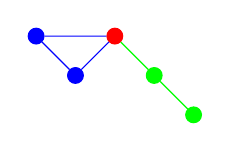
\begin{tikzpicture}[
            vertex/.style={circle, draw, fill=gray!20, minimum size=2mm, inner sep=0pt}
            ]
            \node[vertex,red] (a) at (0,1) {};
            \node[vertex,blue] (b) at (-1,1) {};
            \node[vertex,blue] (c) at (-0.5,0.5) {};
            \node[vertex,green] (d) at (0.5,0.5) {};
            \node[vertex,green] (e) at (1,0) {};
           
            \draw[blue] (b)--(a)--(c)--(b);
            \draw[green] (a)--(d)--(e);
           
            \end{tikzpicture}
            \end{center}
        \item Wlog $G$ is connected.\\
        Assume not ($1$) and $\exists v,v'\in V(G)$ s.t. $G-v-v'$ is disconnected.\\
        Let $C_1',...,C_k'$ be the components of $G-v-v'$. Let $G_i=G[V(C_i')\cup\{v,v'\}]$. Let $G_i'$ be the graph obtained from $G_i$ by adding $\{v,v'\}$ if it is not already there.\\
        Observe that $\forall i\in\{1,...,k\}$, $v$ has a neighbour in $C_i$ (say $v_i'$).\par
              
            \begin{center}
            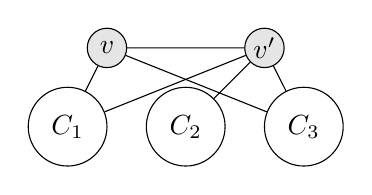
\begin{tikzpicture}[
            vertex/.style={circle, draw, fill=gray!20, minimum size=5mm, inner sep=0pt}
            ]
            \node[vertex] (a) at (-1,1) {$v$};
            \node[vertex] (b) at (1,1) {$v'$};
            \node[circle, draw, fill=white!20, minimum size=10mm, inner sep=0pt] (c) at (-1.5,0) {$C_1$};
            \node[circle, draw, fill=white!20, minimum size=10mm, inner sep=0pt] (d) at (0,0) {$C_2$};
            \node[circle, draw, fill=white!20, minimum size=10mm, inner sep=0pt] (e) at (1.5,0) {$C_3$};
           
            \draw (b)--(a)--(c);
            \draw (c)--(b)--(d);
            \draw (a)--(e)--(b);
            \end{tikzpicture}
            \end{center}
        
        $\deg_{G_i'}(v)=\begin{cases}
            \deg_G(v)-|\bigcup_{j\neq i} N_{C_j}(v)| & \{v,v'\}\in E(G) \\
            \deg_G(v)+1-|\bigcup_{j\neq i} N_{C_j}(v)| & \{v,v'\}\notin E(G)     
            \end{cases}\leq$ \\
            $\begin{cases}
            \Delta(G)-(k-1) & \{v,v'\}\in E(G) \\
            \Delta(G)-(k-2) & \{v,v'\}\notin E(G)
        \end{cases}$   \\
        Same goes for $\deg_{G_i'(v')}$\\
        If $\deg_{G_i'}(v)<\Delta(G)$ or $\deg_{G_i'}(v')<\Delta(G)$, then we can $\Delta(G)$-color $G_i$ by Lemma $(5.4)$.\\
        If $G_1',...,G_k'$ have a $\Delta(G)$-coloring $\implies$ can combine them to a $\Delta(G)$-coloring of $G$.\\
        Suppose $\exists i\in\{1,...k\}$ s.t. $\deg_{G_i'}(v)=\deg_{G_i'}(v')=\Delta(G)$. Wlog $i=2$. Then $k=2, \{v,v'\}\notin E(G)$ ($\deg_{G_i'}(v)<\Delta(G)$ if $k\geq 3$) and $|N_{C_1}(v)|=|N_{C_2}(v')|=1$.\\
        Let $v''\in V(C_1)$ be the neighbour of $v'$\\
        Observation: $\bar G=G-v-v''$ is not connected. $\bar G$ has components $D_1:=C_1-v''$ and $D_2=[V(C_2)\cup \{v'\}]$. $v$ has $\Delta(G)-1$ neighbours in $D_2$ and $v''$ has $\Delta(G)-1$ neighbours in $D_1$. Use the above coloring argument on $G-v-v''$. 
        \begin{center}
            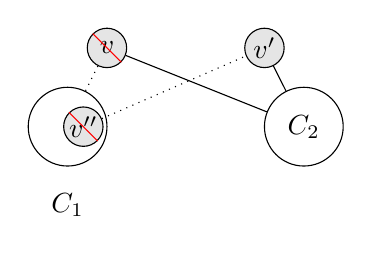
\begin{tikzpicture}[
            vertex/.style={circle, draw, fill=gray!20, minimum size=5mm, inner sep=0pt}
            ]
            \node[vertex] (a) at (-1,1) {$v$};
            \node[vertex] (b) at (1,1) {$v'$};
            \node[circle, draw, fill=white!20, minimum size=10mm, inner sep=0pt] (c) at (-1.5,0) {};
            \node[circle, draw, fill=white!20, minimum size=10mm, inner sep=0pt] (e) at (1.5,0) {$C_2$};
            \node[circle, draw, fill=gray!20, minimum size= 5mm, inner sep=0pt] (f) at  (-1.3,0) {$v''$};
            \node (g) at (-1.5,-1){$C_1$};

            \draw[dotted] (f)--(b);
            \draw[dotted] (a)--(c);
            \draw (a)--(e)--(b);
            \draw[red] (a.north west) -- (a.south east);
            \draw[red] (f.north west) -- (f.south east);
            \end{tikzpicture}
            \end{center}
    \end{enumerate}
\end{proof}